% !Tex program = pdflatex
% 第 2 章: 线性变换 Chap 2: Linear Transform
\ifx\allfiles\undefined
\documentclass{note}
\setcounter{chapter}{+1}
\begin{document}
\fi
\chapter{线性变换}
\section{线性变换}
\begin{df}[线性变换]
    向量空间之间的映射. $F$ 为域, $V,W$ 为 $F$ 上的向量空间, 映射 $\tau:V\rightarrow W$, 若 $\tau(ru+tv)=r\tau(u)+t\tau(v)$, $r,t\in F$, $u,v\in V$, 则称 $\tau$ 为 $V$ 到 $W$ 的线性变换.
\end{df}
(类似于同态)

取 $r=1$, $t=1$, 则 $\tau(u+v)=\tau(u)+\tau(v)$, 故 $\tau$ 是 $V$ 到 $W$ 的群同态, 从而 $\tau(0)=0$, $\tau(-v)=-\tau(v)$.

$\mathcal{L}(V,W)\equiv\{\text{$V$ 到 $W$ 的线性变换}\}$, $\mathcal{L}(V)=\mathcal{L}(V,V)=\{\text{$V$ 到 $V$ 的线性变换}\}=\{\text{$V$ 上的线性算子}\}$.

\begin{df}[单线性变换]
    单射的线性变换.
\end{df}

\begin{df}[满线性变换]
    满射的线性变换.
\end{df}

\begin{df}[同构]
    双射的线性变换. 若两个向量空间 $V,W$ 之间存在同构, 也称这两个向量空间同构, 记作 $V\approx W$.
\end{df}

取 $\tau,\sigma\in\mathcal{L}(V,W)$, $v\overset{\tau}{\mapsto}\tau(v)$, $v\overset{\sigma}{\mapsto}\sigma(v)\Longrightarrow v\overset{\tau+\sigma}{\mapsto}\tau(v)+\sigma(v)$ 也是线性变换, 且 $\tau+\sigma\in\mathcal{L}(V,W)$.
\begin{pf}
    由映射的像的唯一性, $\because v\overset{\tau}{\mapsto}\tau(v)$ 是唯一的, $v\overset{\sigma}{\mapsto}\sigma(v)$ 是唯一的, $\therefore v\overset{\tau+\sigma}{\mapsto}\tau(v)+\sigma(v)$ 是唯一的, 故 $\tau+\sigma$ 是映射.

    $(\tau+\sigma)(ru+tv)=\tau(ru+tv)+\sigma(ru+tv)=r\tau(u)+t\tau(v)+r\sigma(u)+t\sigma(v)=r[\tau(u)+\sigma(u)]+t[\tau(v)+\sigma(v)]=r[(\tau+\sigma)(u)]+t[(\tau+\sigma)(v)]$, 故 $\tau+\sigma$ 为 $V$ 到 $W$ 的线性变换.
\end{pf}
由此定义了线性变换之间的加法.

$(\mathcal{L}(V,W),+)$ 为交换群.
\begin{pf}
    $(\mathcal{L}(V,W),+)$ 满足
    \begin{itemize}
        \item[(1)] \textbf{结合律}: $\forall v\in V$, $[(\tau+\sigma)+\delta](v)=(\tau+\sigma)(v)+\delta(v)=\tau(v)+\sigma(v)+\delta(v)=\tau(v)+(\sigma(v)+\delta(v))=\tau(v)+(\sigma+\delta)(v)=[\tau+(\sigma+\delta)](v)\Longrightarrow[(\tau+\sigma)+\delta]=[\tau+(\sigma+\delta)]$.
        \item[(2)] \textbf{有单位元 $0$}: 零映射 $0(v)=0$, $\forall\tau\in\mathcal{L}(V,W)$, $(0+\tau)(v)=0(v)+\tau(v)=0+\tau(v)=\tau(v)+0=\tau(v)+0(v)=(\tau+0)(v)$.
        \item[(3)] \textbf{有逆元}: $\forall\tau\in\mathcal{L}(V,W)$, $\exists-\tau$, s.t. $(-\tau)(v)=-\tau(v)\Longrightarrow[\tau+(-\tau)](v)=\tau(v)-\tau(v)=0=0(v)$.
        \item[(4)] \textbf{交换律}: $\forall v\in V$, $(\tau+\sigma)(v)=\tau(v)+\sigma(v)=\sigma(v)+\tau(v)=[\sigma+\tau](v)$.
    \end{itemize}
    故 $\mathcal{L}(V,W)$ 为交换群.
\end{pf}

$\forall r\in F$, $v\in\mathcal{L}(V,W)$, $v\overset{\tau}{\mapsto}\tau(v)\Longrightarrow v\overset{r\tau}{\mapsto}r\tau(v)$ 是线性变换, 且 $r\tau\in\mathcal{L}(V,W)$.
\begin{pf}
    由映射的像的唯一性, $\because v\overset{\tau}{\mapsto}\tau(v)$ 是唯一的, $\therefore v\overset{r\tau}{\mapsto}r\tau(v)$ 是唯一的, 故 $r\tau$ 是映射.

    $(r\tau)(v)=r\tau(v)=r[\tau(v)]$, 故 $r\tau$ 为 $V$ 到 $W$ 的线性变换.
\end{pf}

$\mathcal{L}(V,W)$ 是 $F$ 上的向量空间.
\begin{pf}
    前面已证, $(\mathcal{L}(V,W),+)$ 为交换群, 且其满足
    \begin{itemize}
        \item[(1)] $\forall v\in V$, $[(r+t)\tau](v)=(r+t)\tau(v)=r\tau(v)+t\tau(v)=(r\tau+t\tau)(v)\Longrightarrow (r+t)\tau=r\tau+t\tau$
        \item[(2)] $\forall v\in V$, $[(rt)\tau](v)=(rt)\tau(v)=r[t\tau(v)]=[r(t\tau)](v)\Longrightarrow(rt)\tau=r(t\tau)$
        \item[(3)] $\forall v\in V$, $[r(\tau+\sigma)](v)=r(\tau+\sigma)(v)=r[\tau(v)+\sigma(v)]=r\tau(v)+r\sigma(v)=(r\tau+r\sigma)(v)\Longrightarrow r(\tau+\sigma)=r\tau+r\sigma$
        \item[(4)] 恒等映射 $1:\mathcal{L}(V,W)\rightarrow\mathcal{L}(V,W)$, $\tau\overset{1}{\mapsto}$, $\forall v\in V$, $(1\tau)(v)=1[\tau(v)]=\tau(v)\Longrightarrow 1\tau=\tau$
    \end{itemize}
    故得证.
\end{pf}

\begin{thm}[(课本定理 2.1)]
    \begin{itemize}
        \item[(1)] $\mathcal{L}(V,W)$ 是 $F$ 上的向量空间.
        \item[(2)] $t\in\mathcal{L}(V,W)$, $\sigma\in\mathcal{L}(W,U)$, 则 $\sigma\circ\tau\in\mathcal{L}(V,U)$.
        \item[(3)] $\tau$ 是 $V$ 到 $W$ 的同构, 则 $\tau^{-1}\in\mathcal{L}(W,V)$.
        \item[(4)] $\mathcal{L}(V)$ 既是向量空间, 也是环, 且两者的加法运算是一样的, 故 $\mathcal{L}(V)$ 是\textbf{代数}.
    \end{itemize}
\end{thm}

$\mathcal{L}(V)$ 是环.
\begin{pf}
    前面已证, $(\mathcal{L}(V),+)$ 为交换群, 且满足
    \begin{itemize}
        \item[(1)] \textbf{结合律}: $\because$ 映射的复合有结合律, $\therefore\mathcal{L}(V)$ 中元素的复合有结合律
        \item[(2)] \textbf{左右分配律}: $\forall v\in V$, $[(\sigma+\tau)\delta](v)=(\sigma+\tau)[\delta(v)]=\sigma[\delta(v)]+\tau[\delta(v)]=(\sigma\delta)(v)+(\tau\delta)(v)\Longrightarrow(\sigma+\tau)\delta=\sigma\delta+\tau\delta$\\
        $[\sigma(\tau+\delta)](v)=\sigma[(\tau+\delta)(v)]=\sigma[\tau(v)+\delta(v)]=\sigma[\tau(v)]+\sigma[\delta(v)]=\sigma\tau(v)+\sigma\delta(v)\Longrightarrow\sigma(\tau+\delta)=\sigma\tau+\sigma\delta$
    \end{itemize}
    故得证.
\end{pf}

\begin{df}[核空间]
    $\ker\tau\equiv\{v\mid\tau(v)=0\}\subseteq V$.
\end{df}

\begin{df}[像空间]
    $\im\tau\equiv\{\tau(v)\mid v\in V\}$.
\end{df}

\begin{thm}[(课本定理 2.3)]
    \begin{itemize}
        \item[(1)] $\tau$ 满线性变换 $\Longleftrightarrow\im\tau=W$.
        \item[(2)] $\tau$ 单线性变换 $\Longleftrightarrow\ker\tau=\{0\}$.
    \end{itemize}
\end{thm}

\begin{thm}[(课本定理 2.2)]
    $\mathcal{B}$ 是 $V$ 的基, $\tau\in\mathcal{L}(V,W)$, 则 $\tau$ 可由 $\tau$ 在 $\mathcal{B}$ 上的像唯一确定.
\end{thm}
\begin{pf}
    若已知 $\tau(b_i)\forall b_i\in\mathcal{B}$, 则 $\forall v\in V$, $v=\sum_{i=1}^nr_ib_i$, $r_i\in F$, $b_i\in\mathcal{B}$, $n\in\mathbb{Z}^+$\\
    $\Longrightarrow\tau(v)=\tau\left(\sum_{i=1}^nr_ib_i\right)=\sum_{i=1}^nr_i\tau(b_i)$.
\end{pf}

同构的向量空间有很多性质可以相互传递, 下面我们就来讨论这件事.

\begin{thm}[(课本定理 2.4)]\label{thm-2.4}
    $\tau\in\mathcal{L}(V,W)$ 同构, $S$ 是 $V$ 真子集, 则
    \begin{itemize}
        \item[(1)] $V=\langle S\rangle\Longleftrightarrow W=\langle\tau(S)\rangle$.
        \item[(2)] $S$ 线性无关 $\Longleftrightarrow\tau(S)$ 线性无关.
        \item[(3)] $S$ 是 $V$ 的基 $\Longleftrightarrow\tau(S)$ 是 $V$ 的基.
    \end{itemize}
\end{thm}
\begin{pf}
    \begin{itemize}
        \item[(1)] ``$\Longrightarrow$'': $\because V=\langle S\rangle$, $\therefore\forall v\in V$, $v=\sum_ir_is_i$,\\
        又 $\because\tau$ 同构, $\therefore\forall w\in W$, $\exists v\in V$, s.t. $w=\tau(v)\Longrightarrow\tau(v)=\tau\left(\sum_ir_is_i\right)=\sum_ir_i\tau(s_i)$.

        ``$\Longleftarrow$'': $\because W=\langle\tau(S)\rangle$, $\therefore\forall w\in W$, $w=\sum_ir_i\tau(s_i)$,\\
        又 $\because\tau$ 同构, $\therefore\forall v\in W$, $\exists w\in W$, s.t. $v=\tau^{-1}(w)=\tau^{-1}\left(\sum_ir_i\tau(s_i)\right)=\sum_ir_i\tau^{-1}(\tau(s_i))=\sum_ir_i\tau(s_i)$.

        综上, (1) 得证.
        \item[(2)] ``$\Longrightarrow$'': 假设 $\sum_ir_i\tau(s_i)=0$, 则 $\tau\left(\sum_ir_is_i\right)=0$,\\
        又 $\because\tau$ 同构, $\therefore\ker\tau=\{0\}\Longrightarrow\sum_ir_is_i=0$,\\
        又 $\because S$ 线性无关, $\therefore r_i=0\forall i\Longrightarrow\tau(S)$ 线性无关.

        ``$\Longleftarrow$'': 假设 $\sum_ir_is_i=0$, 则 $\tau\left(\sum_ir_is_i\right)=\sum_ir_i\tau(s_i)=0$,\\
        又 $\because\tau(S)$ 线性无关, $\therefore r_i=0\forall i\Longrightarrow S$ 线性无关.

        综上, (2) 得证.
        \item[(3)] (1), (2) $\Longrightarrow$ (3).
    \end{itemize}
\end{pf}

\begin{thm}[(课本定理 2.6)]
    $V\approx W\Longleftrightarrow\dim V=\dim W$.
\end{thm}

\begin{thm}[(课本定理 2.7)]
    若 $\dim V=n$, 则 $V\approx F^n$.
\end{thm}

\begin{thm}[(课本定理 2.8)]
    $\tau\in\mathcal(L)(V,W)$,
    \begin{itemize}
        \item[(1)] $(\ker\tau)^c\approx\im\tau$.
        \item[(2)] $\dim V=\dim\ker\tau+\dim\im\tau\equiv\nul\tau+\rk\tau$, 其中称 $\nul\tau\equiv\dim\ker\tau$ 为 $\tau$ 的零度, $\rk\tau\equiv\dim\im\tau$ 为 $\tau$ 的秩.
    \end{itemize}
\end{thm}
\begin{pf}
    \begin{itemize}
        \item[(1)] 设映射 $\tau^c:\ker(\tau)^c\rightarrow\im\tau$, $u\mapsto\tau(u)$.

        先证 $\tau^c$ 是单射: $\ker(\tau^c)=\ker(\tau)\cap\ker(\tau)^c$ (即 $\ker(\tau^c)$ 中的元素同时满足 $\ker(\tau)$ 的条件, 且在定义域 $\ker(\tau)^c$ 中),\\
        又 $\because V=\ker(\tau)\oplus\ker(\tau)^c$, $\therefore\ker(\tau)\cap\ker(\tau)^c=\{0\}\Longrightarrow\ker(\tau^c)=\{0\}$, 故 $\tau^c$ 单射.

        再证 $\tau^c$ 是满射: 一方面, $\im(\tau^c)\subseteq\im(\tau)$;\\
        另一方面, $\forall\tau(v)$, $v=u+w$, 其中 $u\in\ker(\tau)$, $w\in\ker(\tau)^c\Longrightarrow\tau(v)=\tau(u+w)=\tau(u)+\tau(w)=0+\tau(w)=\tau(w)\in\im(\tau^c)\Longrightarrow\im(\tau)\subseteq\im(\tau^c)$.\\
        故 $\im(\tau^c)=\im(\tau)$, 即 $\tau^c$ 满射.

        综上, (1) 得证.
        \item[(2)] $\dim V=\dim\ker(\tau)+\dim\ker(\tau)^c=\dim\ker(\tau)+\dim\im(\tau)$.
    \end{itemize}
\end{pf}

$x$ 为 $n$ 维向量, $\dim\{x\mid Ax=0\}=n-\rk A$, 故 $\dim\{x\mid Ax=0\}=\nul A$.

\section{表示}
``表示''其实就是用已知的东西展现未知的东西, 在这里, 我们用已知的矩阵乘法展现未知的线性变换, 这就是线性变换的表示.

$F$ 为域, $F^n=\{(r_1,\cdots,r_n)\mid r_i\in F\}$, 满足 $(r_1,\cdots,r_n)+(l_1,\cdots,l_n)=(r_1+l_1,\cdots,r_n+l_n)$ 及 $r(r_1,\cdots,r_n)=(rr_1,\cdots,rr_n)$, $\dim F^n=n$, $F^n$ 的标准基为 $\{e_1=(1,0,\cdots,0),e_2=(0,1,\cdots,0),\cdots,e_n=(0,0,\cdots,1)\}$; $F^m=\{(r_1,\cdots,r_m)\mid r_i\in F\}$, $\dim F=m$, 标准基为 $\{f_1=(1,0,\cdots,0),f_2=(0,1,\cdots,0),\cdots,f_m=(0,0,\cdots,1)\}$. 如何确定/展现 $F^n$ 到 $F^m$ 的线性变换?

根据定理 \ref{thm-2.4}, 我们只需确定一组基在线性变换下的表现, 就可以确定这一线性变换.
\begin{pf}
    $\{b_1,\cdots,b_n\}$ 为 $V$ 的基, 线性变换 $\tau\in\mathcal{L}(V,W)$, 若已知 $\tau(b_i)\forall i$, 则 $\forall v\in V$, $v=\sum_{i=1}^nr_ib_i\Longrightarrow\tau(v)=\tau\left(\sum_{i=1}^nr_ib_i\right)=\sum_{i=1}^nr_i\tau(b_i)$ 可以确定, 由此 $\tau$ 可以确定.
\end{pf}

因此, $\forall\tau\in\mathcal{L}(F^n,F^m)$, 若 $\tau(e_i)=(a_{1i},\cdots,a_{mi})=\sum_{j=1}^ma_{ji}f_j$.\\
$\forall(r_1,\cdots,r_n)\in F^n$,
\begin{align*}
    \tau((r_1,\cdots,r_n))=&\tau\left(\sum_{i=1}^nr_ie_i\right)=\sum_{i=1}^nr_i\tau(e_i)=\sum_{i=1}^nr_i\left(\sum_{j=1}^ma_{ji}f_j\right)=\sum_{j=1}^m\left(\sum_{i=1}^nr_ia_{ji}\right)f_j=\left(\sum_{i=1}^nr_ia_{1i},\cdots,\sum_{i=1}^nr_ia_{mi}\right)\\
    =&\begin{pmatrix}
        a_{11}&a_{12}&\cdots&a_{1n}\\
        a_{21}&a_{22}&\cdots&a_{2n}\\
        \vdots&\vdots&\ddots&\vdots\\
        a_{m1}&a_{m2}&\cdots&a_{mn}
    \end{pmatrix}\begin{pmatrix}
        r_1\\
        r_2\\
        \vdots\\
        r_n
    \end{pmatrix}=\begin{pmatrix}
        \tau(e_1)&\tau(e_2)&\cdots&\tau(e_n)
    \end{pmatrix}\begin{pmatrix}
        r_1\\
        r_2\\
        \vdots\\
        r_n
    \end{pmatrix}=M_{\tau}\begin{pmatrix}
        r_1\\
        r_2\\
        \vdots\\
        r_n
    \end{pmatrix},
\end{align*}
其中 $M_{\tau}=\begin{pmatrix}
    \tau(e_1)&\tau(e_2)&\cdots&\tau(e_n)
\end{pmatrix}$.\\
故 $\forall\vec{r}\in F^n$, $\tau(\vec{r})=M_{\tau}\vec{r}$.

综上:
\begin{align*}
    \boxed{\mathcal{L}(F^n,F^m)\approx M_{m\times n}(F),\quad\tau\mapsto M_{\tau}=\begin{pmatrix}
        \tau(e_1)&\cdots&\tau(e_2)
    \end{pmatrix}}.
\end{align*}

$f:\mathcal{L}(F^n,F^m)\rightarrow M_{m\times n}(F)$, $\tau\mapsto M_{\tau}$ 是线性变换.
\begin{pf}
    由上述的 $M_{\tau}$ 构造过程知, $f(\tau)=M_{\tau}$ 是唯一的, 故 $f$ 是映射.

    \begin{align*}
        f(r\tau+t\sigma)=&M_{r\tau+t\sigma}=\begin{pmatrix}
            (r\tau+t\sigma)(e_1)&\cdots&(r\tau+t\sigma)(e_n)
        \end{pmatrix}=\begin{pmatrix}
            r\tau(e_1)+t\sigma(e_n)&\cdots&r\tau+t\sigma(e_n)
        \end{pmatrix}\\
        =&r\begin{pmatrix}
            \tau(e_1)&\cdots&\tau(e_n)
        \end{pmatrix}+t\begin{pmatrix}
            \sigma(e_1)&\cdots&\sigma(e_n)
        \end{pmatrix}=rM_{\tau}+tM_{\sigma}=rf(\tau)+tf(\sigma).
    \end{align*}
    故 $f$ 是线性的.

    综上, $f:\mathcal{L}(F^n)\rightarrow M_{m\times n}(F)$, $\tau\mapsto M_{\tau}$ 是线性变换.
\end{pf}

f 单射.
\begin{pf}
    $\ker f\equiv\{\tau\mid f(\tau)=0\}=\{\tau\mid M_{\tau}=0\}$.\\
    $\forall\tau\in\ker f$, $\forall\vec{r}\in F^n$, $\tau(\vec{r})=M_{\tau}\vec{r}=\vec{0}\Longrightarrow M_{\tau}=0_{m\times n}\Longrightarrow\tau=0$.\\
    故 $\ker f=\{0\}$ (这里的``$0$''代表的是零变换) $\Longleftrightarrow f$ 单射.
\end{pf}

$f$ 满射.
\begin{pf}
    $\forall A\in M_{m\times n}(F)$, 可由 $\begin{pmatrix}
        \tau(e_1)&\cdots&\tau(e_n)
    \end{pmatrix}=M_{\tau}=A$ 构造 $\tau$, 从而 $f$ 满射.
\end{pf}

综上, $f$ 同构.

取 $V$ 的基 $\mathcal{B}=\{b_1,\cdots,b_n\}$, $\forall v\in V$, $v=\sum_ir_ib_i$.\\
当 $\mathcal{B}$ 定序, $\phi_{\mathcal{B}}:V\rightarrow F^n$, $v\mapsto\begin{pmatrix}
    r_1\\
    \vdots\\
    r_n
\end{pmatrix}\equiv[v]_{\mathcal{B}}$ 是一个映射.
\begin{pf}
    由于 $\mathcal{B}$ 是 $V$ 的基, 展开式 $v=\sum_ir_ib_i$ 唯一确定, 又 $\because\mathcal{B}$ 定序, 从而映射 $v\mapsto\begin{pmatrix}
        r_1\\
        \vdots\\
        r_n
    \end{pmatrix}$ 唯一确定, 故 $\phi_{\mathcal{B}}$ 为映射.

    $\forall u,v\in V$, $u=\sum_{i=1}^nw_ib_i$, $v=\sum_{i=1}^nr_ib_i$,
    \begin{align*}
        \phi_{\mathcal{B}}(r\vec{u}+t\vec{v})=&\phi_{\mathcal{B}}\left(r\left(\sum_{i=1}^nw_ib_i\right)+t\left(\sum_{i=1}^nr_ib_i\right)\right)=\phi_{\mathcal{B}}\left(\sum_{i=1}^n(rw_i+tr_i)b_i\right)=\begin{pmatrix}
            rw_1+tr_1\\
            \vdots\\
            rw_n+tr_n
        \end{pmatrix}\\
        =&r\begin{pmatrix}
            w_1\\
            \vdots\\
            w_n
        \end{pmatrix}+t\begin{pmatrix}
            r_1\\
            \vdots\\
            r_n
        \end{pmatrix}=r\phi_{\mathcal{B}}(u)+t\phi_{\mathcal{B}}(v),
    \end{align*}
    故 $\phi_B$ 为 $V$ 到 $F^n$ 的线性变换.
\end{pf}

$\phi_{\mathcal{B}}$ 单射.
\begin{pf}
    $\ker\phi_{\mathcal{B}}=\{v\mid\phi_{\mathcal{B}}(v)=\begin{pmatrix}
        0\\
        \vdots\\
        0
    \end{pmatrix}\}$.\\
    $\phi_{\mathcal{B}}(v)=\begin{pmatrix}
        0\\
        \vdots\\
        0
    \end{pmatrix}\Longrightarrow v=\sum_{i=1}^n0b_i=0$.\\
    故 $\ker\phi_{\mathcal{B}}=\{0\}\Longleftrightarrow\phi_{\mathcal{B}}$ 单射.
\end{pf}

$\phi_{\mathcal{B}}$ 满射.
\begin{pf}
    $\forall\begin{pmatrix}
        r_1\\
        \vdots\\
        r_n
    \end{pmatrix}\in F^n$, $\exists v\in V$, s.t. $\sum_{i=1}^nr_ib_i\in V$, 故 $\phi_{\mathcal{B}}$ 满射.
\end{pf}

综上, $\phi_{\mathcal{B}}$ 同构.

取 $V$ 的一组定序基 $\mathcal{B}=\{b_1,\cdots,b_n\}$, 另一组定序基 $\mathcal{C}=\{c_1,\cdots,c_n\}$, $v$ 在 $\mathcal{B}$ 下的表象为 $[v]_{\mathcal{B}}$, 在 $\mathcal{C}$ 下的表象为 $[v]_{\mathcal{C}}$, 映射关系见如下的交换图. 如何联系 $v$ 在不同基下的表象, $[v]_{\mathcal{B}}$ 和 $[v]_{\mathcal{C}}$, 从而得到 $\tau$?
\begin{center}
    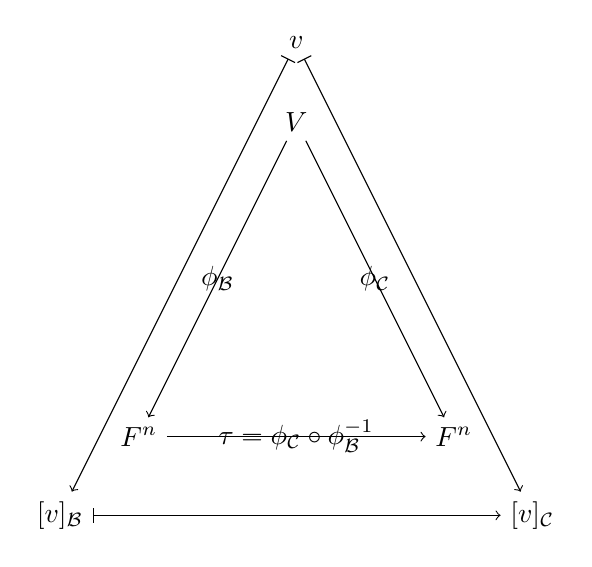
\begin{tikzpicture}
        \node(1)at(0,2){$V$};
        \node(2)at(-2,-2){$F^n$};
        \node(3)at(2,-2){$F^n$};
        \node(4)at(0,3){$v$};
        \node(5)at(-3,-3){$[v]_{\mathcal{B}}$};
        \node(6)at(3,-3){$[v]_{\mathcal{C}}$};
        \draw[->](1)--(2)node[midway]{$\phi_{\mathcal{B}}$};
        \draw[|->](4)--(5);
        \draw[->](1)--(3)node[midway]{$\phi_{\mathcal{C}}$};
        \draw[|->](4)--(6);
        \draw[->](2)--(3)node[midway]{$\tau=\phi_{\mathcal{C}}\circ\phi_{\mathcal{B}}^{-1}$};
        \draw[|->](5)--(6);
    \end{tikzpicture}
\end{center}

$[v]_{\mathcal{C}}=\tau([v]_{\mathcal{B}})=M_{\tau}[v]_{\mathcal{B}}$, 其中 $M_{\tau}=\begin{pmatrix}
    \tau(e_1)&\cdots&\tau(e_n)
\end{pmatrix}$.\\
$\tau:F^n\rightarrow F^n,\quad e_i\mapsto\tau(e_i)=\phi_{\mathcal{C}}(\phi_{\mathcal{B}}^{-1}(e_i))=\phi_{\mathcal{C}}(b_i)$,\\
$M_{\tau}=\begin{pmatrix}
    [b_1]_{\mathcal{C}}&\cdots&[b_n]_{\mathcal{C}}
\end{pmatrix}\equiv M_{\mathcal{BC}}$.

\begin{thm}[(课本定理 2.12)]
    \begin{align*}
        \boxed{[v]_{\mathcal{C}}=M_{\mathcal{BC}}[v]_{\mathcal{B}}}
    \end{align*}
    其中 $[v]_{\mathcal{B}}$ 和 $[v]_{\mathcal{C}}$ 分别是向量 $v$ 在基 $\mathcal{B}$ 和 $\mathcal{C}$ 表象下的坐标表示, $M_{\mathcal{BC}}$ 是在两种坐标表示之间线性变换对应的矩阵.
\end{thm}

\begin{center}
    \begin{tikzpicture}
        \node(1)at(-2,2){$V$};
        \node(2)at(2,2){$W$};
        \node(3)at(-2,-2){$F^n$};
        \node(4)at(2,-2){$F^n$};
        \node(5)at(-3,3){$v$};
        \node(6)at(3,3){$\tau(v)$};
        \node(7)at(-3,-3){$[v]_{\mathcal{B}}$};
        \node(8)at(3,-3){$\tau([v]_{\mathcal{B}})=[v]_{\mathcal{C}}$};
        \node(9)at(-4,4){$b_i$};
        \node(10)at(4,4){$\tau(b_i)$};
        \node(11)at(-4,-4){$e_i$};
        \node(12)at(4,-4){$\tau_A(e_i)=[\tau(b_i)]_{\mathcal{C}}$};
        \draw[->](1)--(2)node[midway]{$\tau$};
        \draw[->](1)--(3)node[midway]{$\phi_{\mathcal{B}}$};
        \draw[->](2)--(4)node[midway]{$\phi_{\mathcal{C}}$};
        \draw[->](3)--(4)node[midway]{$\tau_A=\phi_{\mathcal{C}}\circ\tau\circ\phi_{\mathcal{B}}^{-1}$};
        \draw[|->](5)--(6);
        \draw[|->](5)--(7);
        \draw[|->](6)--(8);
        \draw[|->](7)--(8);
        \draw[|->](9)--(10);
        \draw[|->](9)--(11);
        \draw[|->](10)--(12);
        \draw[|->](11)--(12);
    \end{tikzpicture}
\end{center}
\begin{align*}
    M_{\tau_A}=&\begin{pmatrix}
        \tau_A(e_1)&\cdots&\tau(e_n)
    \end{pmatrix}=\begin{pmatrix}
        \phi_{\mathcal{C}}\circ\tau\circ\phi_{\mathcal{B}}^{-1}(e_1)&\cdots&\phi_{\mathcal{C}}\circ\tau\circ\phi_{\mathcal{B}}^{-1}(e_n)
    \end{pmatrix}=\begin{pmatrix}
        \phi_{\mathcal{C}}\circ\tau(b_1)&\cdots&\phi_{\mathcal{C}}\circ\tau(b_n)
    \end{pmatrix}\\
    =&\begin{pmatrix}
        [\tau(b_1)]_{\mathcal{C}}&\cdots&[\tau(b_n)]_{\mathcal{C}}
    \end{pmatrix}\equiv[\tau]_{{\mathcal{BC}}}.
\end{align*}

\begin{thm}[(课本定理 2.14)]
    \begin{align*}
        \boxed{[\tau(v)]_{\mathcal{C}}=[\tau(v)]_{\mathcal{BC}}[v]_{\mathcal{B}}}
    \end{align*}
    其中 $[\tau(v)]_{\mathcal{C}}$ 是 $\tau(v)$ 在基 $\mathcal{C}$ 的表象下的坐标表示, $[\tau(v)]_{\mathcal{BC}}$ 是从基 $\mathcal{B}$ 的表象到基 $\mathcal{C}$ 的表象的线性变换的矩阵表示, $[v]_{\mathcal{B}}$ 是 $v$ 在基 $\mathcal{B}$ 的表象下的坐标表示.
\end{thm}

\begin{thm}[(课本定理 2.15)]
    $\mathcal{L}(V,W)\rightarrow\mathcal{L}(F^n,F^m)\approx M_{m\times n}(F)$, $\tau\mapsto\tau_A\mapsto[\tau]_{\mathcal{BC}}$.
\end{thm}

若我们改变 $V$ 和 $W$ 的基, 那么映射所联系的向量的坐标会如何?

\begin{center}
    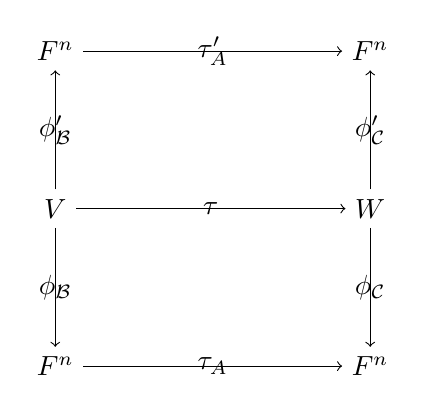
\begin{tikzpicture}
        \node(1)at(-2,0){$V$};
        \node(2)at(2,0){$W$};
        \node(3)at(-2,-2){$F^n$};
        \node(4)at(2,-2){$F^n$};
        \node(5)at(-2,2){$F^n$};
        \node(6)at(2,2){$F^n$};
        \draw[->](1)--(2)node[midway]{$\tau$};
        \draw[->](1)--(3)node[midway]{$\phi_{\mathcal{B}}$};
        \draw[->](2)--(4)node[midway]{$\phi_{\mathcal{C}}$};
        \draw[->](3)--(4)node[midway]{$\tau_A$};
        \draw[->](1)--(5)node[midway]{$\phi_{\mathcal{B}}'$};
        \draw[->](2)--(6)node[midway]{$\phi_{\mathcal{C}}'$};
        \draw[->](5)--(6)node[midway]{$\tau_A'$};
    \end{tikzpicture}
\end{center}

$\tau_A'=\phi_{\mathcal{C}}'\phi_{\mathcal{C}}^{-1}\tau_A\phi_{\mathcal{B}}\phi_{\mathcal{B}}'^{-1}$.

\begin{thm}[(课本定理 2.16)]
    \begin{align*}
        \boxed{[\tau]_{\mathcal{B'C'}}=M_{CC'}[\tau]_{\mathcal{BC}}M_{\mathcal{B'B}}}
    \end{align*}
    其中 $[\tau]_{\mathcal{BC}}$ 和 $[\tau]_{\mathcal{B'C'}}$ 分别是线性变换 $\tau$ 在基 $(\mathcal{B},\mathcal{C})$ 和 $(\mathcal{B}',\mathcal{C}')$ 下的表示, 矩阵 $M_{\mathcal{B'B}}$ 和 $M_{\mathcal{CC}'}$ 分别对应了从基 $\mathcal{B}$ 到基 $\mathcal{B}'$ 和从基 $\mathcal{C}$ 到基 $\mathcal{C}'$ 的变换矩阵.
\end{thm}

$M_{\mathcal{BB}'}$ 可逆.
\begin{pf}
    设 $\phi_{\mathcal{B}}:V\rightarrow F^n$, $v=\sum_{i=1}^nr_ib_i\mapsto[v]_{\mathcal{B}}=\begin{pmatrix}
        r_1\\
        \vdots\\
        r_n
    \end{pmatrix}$ , $\phi_{\mathcal{B}'}:V\rightarrow F^n$, $v=\sum_{i=1}^nr_i'b_i'\mapsto[v]_{\mathcal{B}'}\begin{pmatrix}
        r_1'\\
        \vdots\\
        r_n'
    \end{pmatrix}$, 即
    \begin{center}
        \begin{tikzpicture}
            \node(1)at(0,2){$V$};
            \node(2)at(-2,-2){$F^n$};
            \node(3)at(2,-2){$F^n$};
            \node(4)at(0,3){$v$};
            \node(5)at(-3,-3){$[v]_{\mathcal{B}}$};
            \node(6)at(3,-3){$[v]_{\mathcal{B}'}$};
            \draw[->](1)--(2)node[midway]{$\phi_{\mathcal{B}}$};
            \draw[->](1)--(3)node[midway]{$\phi_{\mathcal{B}'}$};
            \draw[->](2)--(3)node[midway]{$\tau$};
            \draw[|->](4)--(5);
            \draw[|->](4)--(6);
            \draw[|->](5)--(6);
        \end{tikzpicture}
    \end{center}
    $M_{\mathcal{BB}'}=M_{\tau}=\begin{pmatrix}
        [b_1]_{\mathcal{B}'}&\cdots&[b_n]_{\mathcal{B}'}
    \end{pmatrix}$, s.t. $[v]_{\mathcal{B}'}=M_{\mathcal{BB}'}[v]_{\mathcal{B}}$.\\
    同理可以构造 $M_{\mathcal{BB}'}=\begin{pmatrix}
        [b_1']_{\mathcal{B}}&\cdots&[b_n']_{\mathcal{B}}
    \end{pmatrix}$, s.t. $[v]_{\mathcal{B}}=M_{\mathcal{B'B}}[v]_{\mathcal{B}'}$.\\
    $\forall[v]_{\mathcal{B}}\in F^n$, $M_{\mathcal{BB}'}M_{\mathcal{B'B}}[v]_{\mathcal{B}}=M_{\mathcal{BB}'}[v]_{\mathcal{B}'}=[v]_{\mathcal{B}}\Longrightarrow M_{\mathcal{BB}'}M_{\mathcal{B'B}}=n\times n$ 维的单位矩阵, 即 $M_{\mathcal{B'B}}$ 是 $M_{\mathcal{BB}'}$ 的逆, 故 $M_{\mathcal{BB}'}$ 可逆.
\end{pf}

\begin{thm}[(课本定理 2.18)]
    $B=PAQ$, 其中 $P$ 和 $Q$ 可逆, 则 $B$ 与 $A$ \textbf{等价}.
\end{thm}
(因为 $B$ 和 $A$ 是同一线性变换在两组不同的基下的表示.)

\begin{thm}[(课本定理 2.19)]
    $B=PAP^{-1}$, 其中 $P$ 可逆, 则 $B$ 与 $A$ \textbf{相似}.
\end{thm}
(因为 $B$ 和 $A$ 是同一线性算子在两组不同的基下的表示.)
\ifx\allfiles\undefined
\end{document}
\fi